input{preamble.tex}


\title{Software Innovation: Miniproject}
\author{Jacob Karsten Wortmann\\Jesper Riemer Andersen\\Nicklas Andersen\\Sam Sepstrup Olesen\\Simon Reedtz Olesen}

\begin{document}
\maketitle

\subsection*{Brief description}
The idea of the project is to make an interactive cookbook on the android platform that can give you suggestions of recipes based on chosen ingredients. An advantage of the interactive recipe search based on ingredients could be that whenever you find an interesting ingredient in the store, you can choose this ingredient in the application and quickly get relevant suggestions of recipes and thereby identify which additional ingredients you need to buy. Another use for this functionality is to find interesting recipes that you can make with the ingredients you already have at home or few additional ingredients.

\subsection*{Challenges}
The main challenge of the project is to make an efficient search algorithm that rivals the other similar applications on the market. The problem with the other existing solutions is that if you for example input ``eggs'' and ``chicken'', you will get many different recipes of how to prepare eggs, and not on how to combine the two ingredients. The overall design of the application can also prove to be a major challenge because we have to fit a large amount of information on a relatively small mobile screen.

\section*{Section 1}
% a brief description of your initial project idea at the start of the semester (no more than half a page).

\subsection*{Problem Domain}

When a user stands in their kitchen or in the supermarket and wants to look up a recipe for dinner, they must be able to access this easily.

Our application focuses on making it easy to access recipes on mobile devices. We want to split up the recipes in core and optional ingredients, in order to optimise the search results the user gets. For this we need to analyse each recipe that will be used in the application.

\subsection*{Use Context}

The application can be used in different scenarios, for example the user can be at home and type in the items they have in their kitchen to get suggestions for that recipes they can use. The user can also stand in the supermarket and see an item on sale and use the interactive system to find which recipes they can make with that item and what other items they also need to buy. 

\paragraph{Metaphor}

A metaphor for our application could be a cookbook on your mobile phone. 

\paragraph{Focus on the Essentials}

\subsection*{Affordance}

\begin{description}

\item [Navigation drawer] is a feature in Android, allowing the user to swipe from the left of the screen and open a "drawer" with different views that they can navigate to. Navigation drawer is standard design pattern in Android so this design will behave in a consistent and predictable fashion known to the user.
\item [Action bar] is also a feature in Android. Like the navigation drawer this is also a standard design pattern. This is where the user expects the actions to be, so this is the natural placement of our search function. The action bar also shows that the navigation drawer is available and it can also open it since it is an action. 
\item[Scrolling] is a basic feature in almost every application in order to show more information than what fits on the screen. The scrolling feature is usually indicated by partially displaying the content at the bottom or at either side.

\end{description}

\subsection*{Evaluation Criteria}

The application must be fast to use, it must also have a low learning curve.

\subsection*{Prototype configuration}

\subsection*{Story, Julie}

Julie is at the supermarket, she does not know what to have for dinner later. She sees that minced beef is on sale, but she does not know what recipes include this. She opens the application. She is presented with a page that says "Click above to search for ingredients". She clicks the button, and a view of categories appears at the bottom of the screen. She clicks the category called "Meat", and a word cloud appears with many different kinds of meat. In the word cloud she finds minced beef and clicks it. She now dismisses the ingredient search, and the application now presents Julie with recipes which uses minced beef. The top results include recipes such as Spaghetti Bolognese and Lasagne. Having not thought about this before, Julie wants to cook Spaghetti Bolognese for dinner. She opens the recipe and can now see all the ingredients she need for this recipe. Remembering which of the ingredients she has at home, she then adds the ingredients she needs to her shopping list. Then she favourites the recipe to easily find it later. Julie opens her shopping list and continues shopping.


\begin{figure}[H]
\begin{minipage}[b]{0.5\columnwidth}
\centering
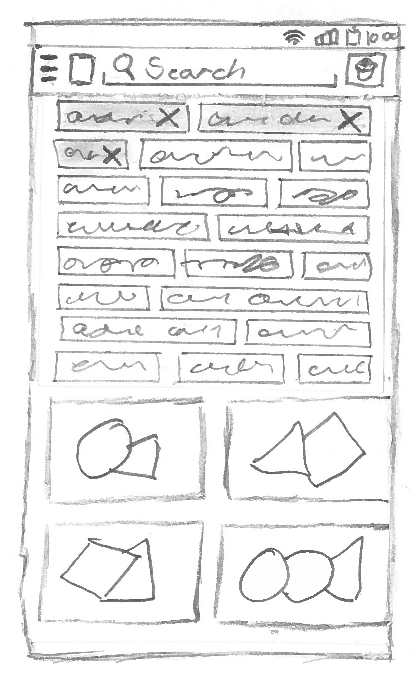
\includegraphics[width=0.7\columnwidth]{../img/prototypes/ingredient_search_tile.pdf}
\caption{Ingredient search with tile selection\label{fig:ingreani}}
\end{minipage}
\hspace{0.5cm}
\begin{minipage}[b]{0.5\columnwidth}
\centering
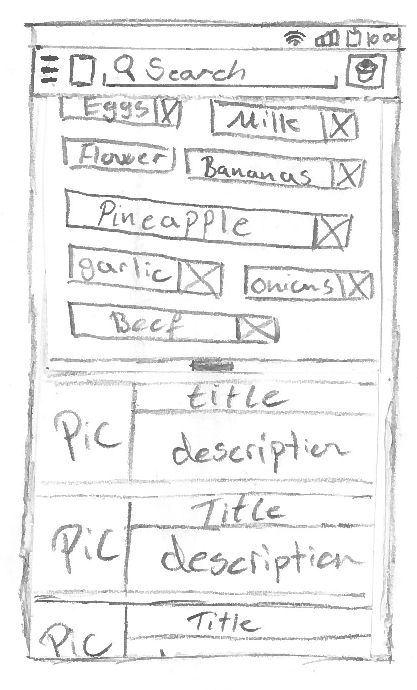
\includegraphics[width=0.72\columnwidth]{../img/prototypes/recipe_browse2.pdf}
\caption{Recipe browsing with selected ingredients \label{fig:recipeword}}
\end{minipage}
\end{figure}

The vision for the project is to digitalise a cookbook so users easily can search for recipes and find instruction for dishes. 

\autoref{fig:ingreani} shows the ingredient search page. The idea with the design is so the user can quickly navigate to the ingredient they want with a few presses. This makes it easier to find ingredients with one hand, which is common when you are out shopping and you have a basket in one hand. The user starts searching by clicking the search field at the top, which is indicated with the ``Magnifying glass''. When the user starts searching a word cloud appear. The functionality of the word cloud is to suggest ingredients to the user based on the ingredients they already put in. This should help the user to quickly add the ingredients they want. 

The problem with this design is if the user prefers to search by text, or perhaps it is too hard for the user to figure out what category the item they are looking for belongs to. Therefore it would be ideal to also have a way for the user to type in their recipes using a keyboard and text and some sort of autocomplete to help the user.

\autoref{fig:recipeword} shows the recipe browse page. There the user has an overview of the recipes that matches his ingredients. The user can still see the ingredients they put in which allows them to quickly add or remove ingredients from their search. However, the view is very small so the user cannot see many recipes at a time. This could be changed by removing the ingredient view when browsing the recipes and then the user would have to click the search field again in order to add or remove ingredients, or the ingredients could be hidden when you scroll up and down, allowing the user a full view of recipes when scrolling but see their inputted ingredients when not. 

\subsection*{Story, Alice}

Alice is at home, earlier she found a Lasagne recipe and she has already bought all the ingredients for it. She opens the application, goes to the favourites page, and opens her previously favourited recipe for Lasagne. In the recipe she scrolls down to the instructions and follows these in order to make her dinner.


\begin{figure}[H]
\begin{minipage}[b]{0.5\columnwidth}
\centering
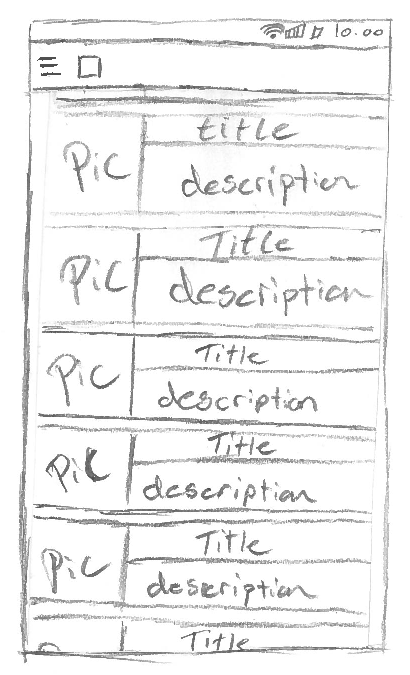
\includegraphics[width=0.7\columnwidth]{../img/prototypes/favorites.pdf}
\caption{The layout for favourites\label{fig:favourite}}
\end{minipage}
\hspace{0.5cm}
\begin{minipage}[b]{0.5\columnwidth}
\centering
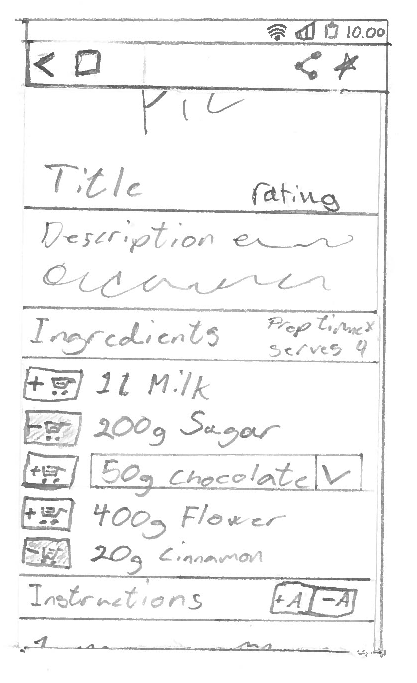
\includegraphics[width=0.735\columnwidth]{../img/prototypes/recipe_new.pdf}
\caption{Redesigned recipe layout\label{fig:recipenew}}
\end{minipage}
\end{figure}

The user must be able to bookmark recipes in order to find them fast when they have to use them.

\autoref{fig:favourite} shows the favourite list. The favourite list is a list of recipes, which allows the user to quickly navigate between them. The simply press the recipe they want to look at and they are taken to it. The recipe page can be seen on \autoref{fig:recipenew}. 

The layout for favourites is very simple and it looks like the page where you browse recipes after having searched. The similar look can be a good thing, since the user is familiar with the layout so they know what happens when you click a recipe.

The recipe consists of a picture of the dish, a title and a rating. Under the picture there is a short description. Then a list of ingredients and the list of instruction the user has to follow. If any of the ingredients can be exchanged with something else, there is a box around it and a drop down menu where you can choose one of the other ingredients.

All the information the user gets on the recipe page might seem cluttered for the user until they learn to use the system. Perhaps the first time the user uses the application a small introduction could be shown, displaying the different functionalities in the application.

\section*{Section 2}
% work-products from using Essence. You can use results from the exercises, but you may also use later material from your project work. The work-products must relate to all four Views in Essence: Paradigm (scenarios, states, prototype), Product (design ideas, technological options), Project (Toulmin structure, other representations of visions, research visions, feature list), and Process (SWOT evaluation and one or both of these: value analysis, use criteria). Work-products in italics are recommended but not mandatory. Provide enough information in this section to illuminate and substantiate your observations in the rest of the presentation.



\section*{Section 3}
% description of how your results developed from your initial project idea (the problem you started out to solve) to status at the time of writing this mini-project. Were there any important leaps in your visions, product ideas, or perceptions of use context?


\section*{Section 4}
% theoretical evaluation

\end{document}